\documentclass[../main.tex]{subfiles}
\graphicspath{{\subfix{../images/}}}
\begin{document}

\subsection{Convolutional Neural Network Model}

The Convolutional Neural Network Model (CNN) iterates on the MLP model by using a 3 dimensional array as its input and using convolution layers. Convolution layers extract features within data by running a kernels across the image to discover features like edges and shapes. Pools were used to reduce the dimension of the images by grouping multiple pixels into a single pixel. 

To iterate on the baseline model, one convolutional layer that extracts 6 layers is added with an additional 2x2 MaxPool which keeps the highest value pixel in a 2x2 pixel area.

\begin{figure}[h!]
  \centering
  \begin{subfigure}[b]{0.35\linewidth}
    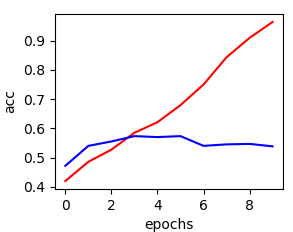
\includegraphics[width=\linewidth]{cnn-performance.png}
  \end{subfigure}
  \caption{Performance of the CNN}
  \label{fig:cnn-performance}
\end{figure}

In Figure \ref{fig:cnn-performance}, when the accuracy of the model reached close to 100\% in 9 epochs, the accuracy of the validation remained close to 50\% which indicates model overfitting. We see that the accuracy of the 2 models start to diverge around 4 epochs where overfitting began to occur. 

\end{document}